\section{Docker Architecture}
\label{sec::arch}

% 3. Docker Architecture
%     1. The Docker engine
%         1. Client server
%         2. Monolithic architecture
%         3. runc
%         4. containerd
%     2. Images
%         1. Layers
%         2. Dockerfile
%         3. Docker compose
%     3. Containers
%         1. Container creation process
%         2. Workflow
%     5. Volumes and persistent data
%     6. Networking

\subsection{The Docker Engine}
\label{sec::arch:engine}
The Docker Engine is the core software responsible for running and managing containers, which consists of several modular components following \ac{OCI} specifications\cite{Docker-engine}. It is implemented as a client-server application, consisting in the following components:

\begin{itemize}
    \item A server running the daemon process \texttt{dockerd};
    \item Docker's \acs{REST}ful \ac{API};
    \item The \ac{CLI} client, \texttt{docker}.
\end{itemize}

In this model, the Docker daemon is the component responsible for creating, running and managing the containers. The daemon is able to manage any number of containers in the device, all controlled via the \ac{CLI} interface. The client interacts with the Docker daemon via its own \ac{REST} \ac{API} over Unix sockets or a network interface\cite{Poulton2020-ju}.

\begin{figure}[!htb]
    \centering
    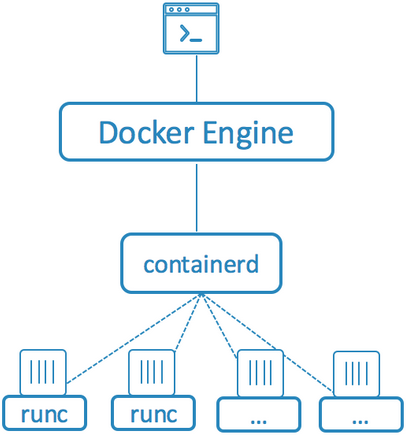
\includegraphics[width=0.25\textwidth]{docker_engine.png}
    \caption{Current and planned container use for all organizations.}
    \label{fig:docker-engine-server}
\end{figure}

Despite being, at its core, a client-server architecture, Docker's server is far from monolithic, as shown in figure \ref{fig:docker-engine-server}. The server operates a set of smaller components, among them \texttt{runc} and \texttt{containerd} --- the main modules responsible for creating and running containers, both of them implement as closely as possible the \ac{OCI} specifications\cite{Poulton2020-ju}.

\texttt{runc} is a \ac{CLI} component responsible for creating and running applications according to the \ac{OCI} runtime specifications \cite{oci-runc}, which is a open source project and available at \cite{git-runc}. Its purpose is to be a standalone low-level tool called by any high-level application, such as Docker. In order to achive this, \texttt{runc} relies on the library \texttt{libcontainer} to access the container isolation features of the \ac{OS}, such as \texttt{seccomp} and user namespaces\cite{runc-estes}.

\texttt{containerd} is responsible for managing all the container execution logic, such as starting, stopping and removing containers. In the same way as \texttt{runc}, \texttt{containerd} is available as a standalone daemon and was intended to be a lightweight program with the sole role of managing container lifetime operations. But as it grew, it gained new functionalities, such as data storage and image management\cite{docker-containerd}.

\placeholder{With this in mind, explain the dockers container creation workflow.}
When a command is typed into de \ac{CLI}, the Docker client converts the instructions into the \ac{API} payload and POSTs to the correct API endpoint. Once the daemon receives the command to create a new containers, a call is made to \texttt{containerd}, which converts the required Docker Image into a bundle and instructs \texttt{runc} to create a new container. \texttt{runc} in its turn, interfaces with the \ac{OS} kernel to allocate the resources and to execute the instructions needed to create a new container. The container process is started as a child-process of \texttt{runc}, and as soon as it is started, \texttt{runc} is terminated.

\subsection{Containers}
\label{sec::arch:containers}
As defined by the \texttt{libcontainer} README page \cite{docker-libcontainer}, a container is "a self-contained execution environment that shares the kernel of the host system and is optionally isolated from other containers in the system".

Despite the behavior similarities between containers and \acp{VM}, they are fundamentally different, since all the containers running in the system share the same kernel, so the isolation between workloads is implemented within that one kernel. As a result, there is one less layer of abstraction between the isolated task and the hardware underneath, which results in better resource efficiency.

How ever, it's only possible to run processes that are compatible with the underlining kernel, i.e. a Windows container cannot run Linux application and vice versa.

\subsection{Container Lifecycle}

% containers follow the same process group signal propagations that any other process group would recieve on linux
% auto restarting a continer?
% normal docker stop sends a SIGTERM to kill the container
% docker stop initially sends sigterm signal, if the container as not stopped within 25 seconds, a SIGKILL signal is sent to forcefully kill it
% if docker kill wont stop the container, docker kill is used

\subsection{Images}
\label{sec::arch:images}
Docker images are a template of what is reconstructed into a running container, it serves as a base for everything that will be deployed and ran on the container, similarly to a filesystem \cite{Kane2018-fn}. Before launching a container, the image must be built from scratch or downloaded from a public registry. When the \texttt{docker pull} command is used, the default registry used is the official Docker Hub \cite{docker-hub}.

An image consists of multiple read-only layer, in which each layer represents the changes made to the underlining system, representing a \texttt{diff} of the previous layer \cite{images-layers}. When a container is created, a new read-write layer is added on top of the previous ones, so that all the changes made during the container execution are saved on disk \cite{fig-src:image-layers}. An example of a docker image composition is shown in the diagram \ref{fig:docker-image}.

In its turn, a layer is identified by a digest, referred to as Content Addressable IDs, as each hash represents the image content. By separating the layers in this fashion, it allows several images to address the same layer, which only needs to be stored once in the device.

\begin{figure}[!htb]
    \centering
    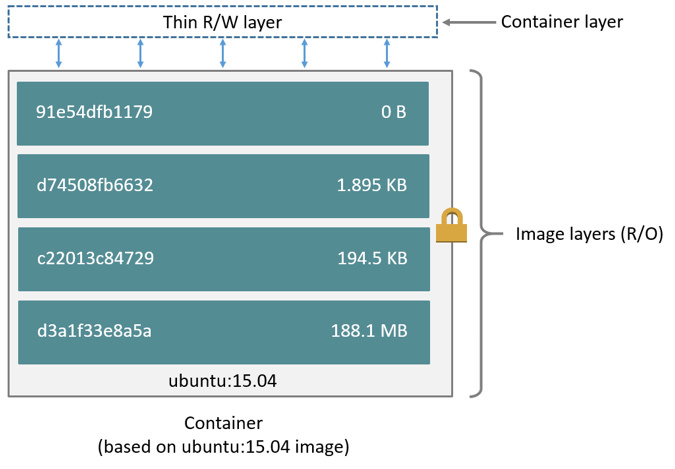
\includegraphics[width=0.45\textwidth]{container-layers.jpg}
    \caption{Layers that compose a Ubuntu container \cite{fig-src:image-layers}.}
    \label{fig:docker-image}
\end{figure}

% image tags
% The manifest list is exactly what it sounds like: a list of architectures supported by a particular image tag. Each supported architecture then has its own *manifest detailing the layers it’s composed from. Figure 6.9 uses the official golang image as an example. On the left is the manifest list with entries for each architecture the image supports. The arrows show that each entry in the manifest list points to a manifest containing image config and layer data. [Docker deep dive]

% manifest list
% Dockerfile
% Docker compose

\subsection{Volumes and Persistent Data}
\label{sec::arch:volumes}

\subsection{Networking}
\label{sec::arch:net}
